\documentclass{oblivoir}
\usepackage{amsmath,amssymb,amsthm,kotex,paralist}

\usepackage[skipabove=10pt,innertopmargin=10pt]{mdframed}

\usepackage{tabto,pifont}
\TabPositions{0.2\textwidth,0.4\textwidth,0.6\textwidth,0.8\textwidth}
\newcommand\tabb[5]{\par\bigskip\noindent
\ding{172}\:{\ensuremath{#1}}
\tab\ding{173}\:\:{\ensuremath{#2}}
\tab\ding{174}\:\:{\ensuremath{#3}}
\tab\ding{175}\:\:{\ensuremath{#4}}
\tab\ding{176}\:\:{\ensuremath{#5}}}

\usepackage{enumitem}
\setlist[enumerate]{label=(\arabic*)}

\newcounter{num}
\newcommand{\defi}[1]
{\noindent\refstepcounter{num}\textbf{정의 \arabic{num}) #1}\par\noindent}
\newcommand{\theo}[1]
{\noindent\refstepcounter{num}\textbf{정리 \arabic{num}) #1}\par\noindent}
\newcommand{\exam}[1]
{\bigskip\bigskip\noindent\refstepcounter{num}\textbf{예시 \arabic{num}) #1}\par\noindent}
\newcommand{\prob}[1]
{\bigskip\bigskip\noindent\refstepcounter{num}\textbf{문제 \arabic{num}) #1}\par\noindent}
\newcommand{\proo}
{\bigskip\textsf{증명)}\par}

\newcommand{\ans}{
{\par
\raggedleft\textbf{답 : (\qquad\qquad\qquad\qquad\qquad\qquad)}
\par}\bigskip\bigskip}

\newcommand{\pb}[1]%\Phantom + fBox
{\fbox{\phantom{\ensuremath{#1}}}}

\newcommand\ba{\;|\;}

\let\oldsection\section
\renewcommand\section{\clearpage\oldsection}

%%%%
\begin{document}

\title{윤영 : 06 집합(1)}
\author{}
\date{\today}
\maketitle
\tableofcontents
\newpage

%%

%%
\section{집합의 뜻}
\begin{mdframed}
%
\defi{집합과 원소}
어떤 조건이나 기준에 의하여 그 대상을 분명히 알 수 있는 것들의 모임을 \textbf{집합}이라고 한다.
또 집합을 이루는 대상 하나하나를 그 집합의 \textbf{원소}라고 한다.
\end{mdframed}

%
\exam{}\label{set_example}
`\(6\)의 약수의 모임'은 그 대상이 \(1\), \(2\), \(3\), \(6\)으로 분명하기 때문에 집합이다.
이때 \(1\), \(2\), \(3\), \(6\)은 원소이다.

%
\prob{}
\begin{enumerate}
\item
\(10\)보다 작은 자연수의 모임	\tabto{0.6\textwidth}(집합이다, 집합이 아니다)
\item
\(1\)에 가까운 수의 모임		\tabto{0.6\textwidth}(집합이다, 집합이 아니다)
\item
성북구에 위치한 중학교의 모임	\tabto{0.6\textwidth}(집합이다, 집합이 아니다)
\item
수학 점수가 높은 학생의 모임	\tabto{0.6\textwidth}(집합이다, 집합이 아니다)
\end{enumerate}

\begin{mdframed}
%
\defi{}
\(a\)가 집합 \(A\)의 원소일 때, `\(a\)는 집합 \(A\)에 속한다'라고 말하고
\[a\in A\]
로 나타낸다.
반대로 \(a\)가 집합 \(A\)의 원소가 아니면 `\(a\)는 집합 \(A\)에 속하지 않는다'라고 말하며
\[a\notin A\]
로 나타낸다.

또한, 원소가 하나도 없는 집합을 \textbf{공집합}이라고 하고 기호로는
\[\varnothing\]
로 나타낸다.
\end{mdframed}

%
\exam{}
예시 \ref{set_example}의 집합을 \(A\)라고 하면
\(1\in A\)이고 \(3\in A\)이다.
그리고 \(4\notin A\)이다.

%
\prob{}
10보다 작은 자연수의 집합을 \(A\)라고 할 때, 다음 빈 칸에 \(\in\), \(\notin\) 중 알맞은 기호를 써넣어라.
\begin{enumerate}
\item
\(0\:\:\pb{\in}\:\:A\)
\item
\(1\:\:\pb{\in}\:\:A\)
\item
\(7\:\:\pb{\in}\:\:A\)
\item
\(13\:\:\pb{\in}\:\:A\)
\item
\(5\:\:\pb{\in}\:\:\varnothing\)
\end{enumerate}

\section{집합의 표현}
%
\exam{}\label{set_notation_example}
%\(A\)를 `8의 약수들의 집합'이라고 할 때, 집합 \(A\)를 나타내는 방법에 대해 알아보자.
\(A\)를 `8의 약수들의 집합'이라고 하자.
\(A\)는 다음의 세 방법으로 나타낼 수 있다.
\begin{enumerate}
\item
\(A\)의 원소들을 일일이 나열하는 방법;
\[A=\{1,2,4,8\}\]
\item
\(A\)에 속하는 조건을 제시하는 방법;
\[A=\{x\;|\;x\text{는 8의 약수}\}\]
\item
그림으로 표현하는 방법;\\
\begin{center}
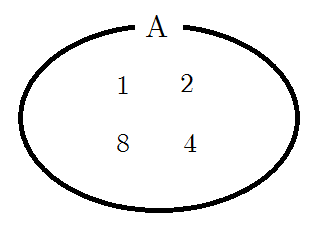
\includegraphics[width=0.3\textwidth]{venn}
\end{center}
\end{enumerate}

\begin{mdframed}
%
\defi{집합의 표현}
집합은 예시 \ref{set_notation_example}의 세 가지 방식으로 표현될 수 있다.
(1)의 방법을 \textbf{원소나열법}, (2)의 방법을 \textbf{조건제시법}이라고 부른다.
(3)의 그림은 \textbf{벤 다이어그램}(Venn diagram)이라고 부른다.
\end{mdframed}

%
\exam{}
\begin{enumerate}
\item
집합\(\{x\ba x\text{는 5 이하의 자연수}\}\)는 원소나열법으로 \(\{1,2,3,4,5\}\)와 같이 나타낼 수 있다.
\item
집합 \(\{5,10,15,20,\cdots\}\)는 \(\{x\ba x\text{는 5의 배수}\}\)
로 나타낼 수 있다.
아니면 \(\{5k\ba k\text{는 자연수}\}\)
로 나타낼 수도 있다.
\end{enumerate}

%
\prob{}
다음 집합을 원소나열법으로 나타내어라.
\begin{enumerate}
\item
\(10\)보다 작은 소수의 집합 \(=\)
\item
\(18\)의 약수의 집합 \(=\)
\item
\(\{x\ba6<x<12,\:\:x\text{는 짝수}\}=\)
\item
\(\{x\ba x\text{는 100 이하의 자연수}\}=\)
\item
\(\{y\ba y\text{는 홀수}\}=\)
\item
\(\{3k-1\ba k\text{는 5 이하의 자연수}\}=\)
\end{enumerate}

%
\prob{}
다음 집합을 조건제시법으로 나타내어라.
\begin{enumerate}
\item
\(\{3,6,9,12,15,18\}=\)
\item
\(\{1,3,5,\cdots,99\}=\)
\item
\(\{\frac12,\frac13,\frac14,\cdots\}=\)
\end{enumerate}

%
\prob{}
다음 집합을 벤 다이어그램으로 나타내어라.
\begin{enumerate}
\item
방정식 \(x^2-4x+3=0\)의 해의 집합 \(A\)
\vspace{0.15\textheight}
\item
\(30\)과 서로소인 \(20\)이하의 자연수의 집합 \(B\)
\vspace{0.15\textheight}
\end{enumerate}

%%
%\prob{}
%다음 세 집합을 비교해보자.
%\begin{align*}
%A&=\{1,3,5\}\\
%B&=\{1,5,3\}\\
%C&=\{1,1,3,5\}
%\end{align*}

%%
\section{부분집합}

\begin{mdframed}
%
\defi{부분집합}
%두 집합 \(A\), \(B\)에 대해서
집합 \(A\)의 모든 원소가 집합 \(B\)에 속할 때, \(A\)를 \(B\)의 \textbf{부분집합}이라고 부른다.
이때 `\(A\)가 \(B\)에 포함된다' 혹은 `\(B\)가 \(A\)를 포함한다'고 말하며 기호로
\[A\subset B\]
와 같이 나타낸다.
또 \(A\)가 \(B\)의 부분집합이 아니면 기호로
\[A\not\subset B\]
와 같이 나타낸다.
\end{mdframed}

%
\exam{}
\begin{enumerate}
\item
두 집합 \(A=\{1,3,5\}\), \(B=\{1,2,3,4,5\}\)에 대하여 \(A\subset B\)이다.
\item
두 집합 \(C=\{2,3,4\}\), \(D=\{3,4,5\}\)에 대하여 \(C\not\subset D\), \(D\not\subset C\)이다.
\end{enumerate}

\begin{center}
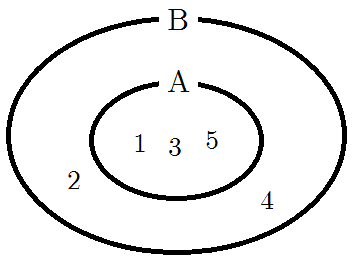
\includegraphics[width=0.3\textwidth]{inclusion_1}
~
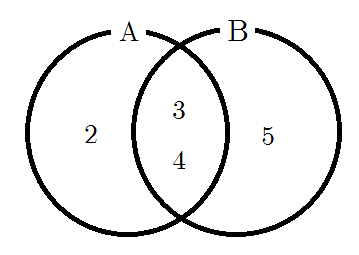
\includegraphics[width=0.3\textwidth]{inclusion_2}

(1)\qquad\qquad\qquad\qquad\qquad(2)
\end{center}

\clearpage
%
\prob{}
다음 두 집합을 벤 다이어그램으로 표현해보고, 빈칸에 \(\subset\), \(\not\subset\) 중 알맞은 기호를 써넣어라.
\begin{enumerate}
\item
\(A=\{1,2,3,4,5\}\), \tabto{0.48\textwidth}\(B=\{x\ba x\text{는 7보다 작은 자연수}\}\)
\vspace{0.18\textheight}
{\par\raggedleft{\textbf{답 : }
A\:\:\pb{\neq}\:\:B,\quad B\:\:\pb{\neq}\:\:A}\par}\bigskip\bigskip
\item
\(A=\{x\ba x\text{는 20 이하의 2의 배수}\}\), 
\tabto{0.48\textwidth}\(B=\{x\ba x\text{는 20 이하의 3의 배수}\}\)
\vspace{0.18\textheight}
{\par\raggedleft{\textbf{답 : }
A\:\:\pb{\neq}\:\:B,\quad B\:\:\pb{\neq}\:\:A}\par}\bigskip\bigskip
\item
\(A=\{3k\ba k\text{는 6 이하의 자연수}\}\), 
\tabto{0.48\textwidth}\(B=\{x\ba x\text{는 20 이하의 3의 배수}\}\)
\vspace{0.18\textheight}
{\par\raggedleft{\textbf{답 : }
A\:\:\pb{\neq}\:\:B,\quad B\:\:\pb{\neq}\:\:A}\par}\bigskip\bigskip
\end{enumerate}


\begin{mdframed}
%
\defi{}
두 집합 \(A\), \(B\)에 대해서 \(A\subset B\), \(B\subset A\)가 동시에 성립할 때, `두 집합 \(A\)와 \(B\)는 서로 같다'라고 말하고, 기호로 
\[A=B\]
와 같이 나타낸다.
또 \(A\subset B\)이고 \(A\neq B\)이면 \(A\)를 \(B\)의 \textbf{진부분집합}이라고 부른다.
\end{mdframed}

\vspace{-10pt}
%
\prob{}
다음 두 집합 \(A\), \(B\)에 대하여 집합 \(A\)가 집합 \(B\)의 진부분집합인 것을 말하여라.
\begin{enumerate}
\item
\(A=\{x\ba x\text{는 8의 약수}\}\), \tabto{0.48\textwidth}\(B=\{1,2,4,8\}\)
\item
\(A=\{x\ba x\text{는 자연수}\}\), \tabto{0.48\textwidth}\(B=\{x\ba x\text{는 정수}\}\)
\end{enumerate}
\vspace{10pt}

%
\exam{}
세 집합 \(A=\{1,2,3\}\), \(B=\{1,3,2\}\), \(C=\{1,1,2,3\}\)에 대하여 \(A\subset B\)이고 \(B\subset A\)이다.
따라서 \(A=B\)이다.
또, \(A\subset C\)이고 \(C\subset A\)이다.
따라서 \(A=C\)이다.

\bigskip
정리하면
\begin{enumerate}
\item
집합에서 원소의 순서가 바뀌어도 같은 집합이다.
\item
중복된 원소는 하나의 원소로 생각한다.
\end{enumerate}

%\begin{align*}
%A&=\{1,3\}\\
%B&=\{1,3,4\}\\
%C&=\{1,2,3,4\}\\
%%D&=\{x\ba (x-1)(x-3)=0\}
%\end{align*}
%\begin{enumerate}
%\item
%\(A\subset A\)
%\item
%\(\varnothing\subset A\)
%\item
%\(A\subset B\)
%\item
%\(B\subset C\)
%\item
%\(A\subset C\)
%\item
%\(B\)는 \(D\)의 진부분집합이다.
%\end{enumerate}

\clearpage
\begin{mdframed}
%
\theo{부분집합의 성질}
세 집합 \(A\), \(B\), \(C\)에 대하여
\begin{enumerate}[label=(\emph{\alph*})]
\item
\(A\subset A\), \(\varnothing\subset A\)
\item
\(A\subset B\)이고 \(B\subset A\)이면 \(A=B\)이다.
\item
\(A\subset B\)이고 \(B\subset C\)이면 \(A\subset C\)이다.
\end{enumerate}
\end{mdframed}

\proo
\((a)\), \((b)\)는 당연하다.
\((c)\)에서 \(A\subset B\)이고 \(B\subset C\)이면 벤 다이어그램이 아래와 같다.

\begin{figure}[h!]
\centering
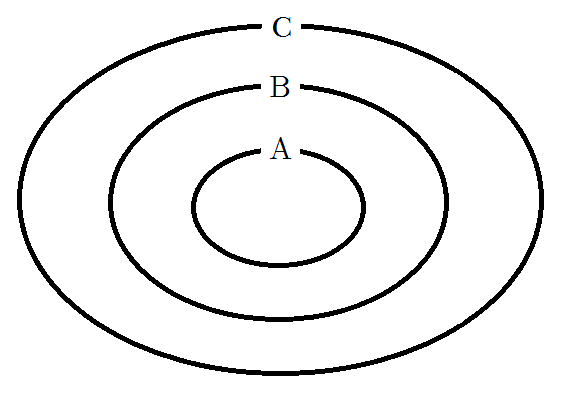
\includegraphics[width=0.4\textwidth]{transitivity}
\end{figure}

따라서 \(A\subset C\)이다.

\clearpage
%
\prob{}\label{number_of_subsets_1}
다음 집합의 부분집합을 모두 구하고, 그 개수를 말하여라.
\begin{enumerate}
\item
\(A=\{a\}\)
\vspace{0.1\textheight}
{\par\raggedleft{\textbf{(\qquad\qquad) 개}}\par}\bigskip\bigskip
\item
\(B=\{a,b\}\)
\vspace{0.1\textheight}
{\par\raggedleft{\textbf{(\qquad\qquad) 개}}\par}\bigskip\bigskip
\item
\(C=\{a,b,c\}\)
\vspace{0.1\textheight}
{\par\raggedleft{\textbf{(\qquad\qquad) 개}}\par}\bigskip\bigskip
\item
\(D=\{a,b,c,d\}\)
\vspace{0.1\textheight}
{\par\raggedleft{\textbf{(\qquad\qquad) 개}}\par}\bigskip\bigskip
\end{enumerate}

%
\prob{}\label{number_of_subsets_2}
문제 \ref{number_of_subsets_1}를 바탕으로 다음 집합의 부분집합의 개수를 유추하여라.
\begin{enumerate}
\item
\(E=\{a,b,c,d,e\}\)
{\par\raggedleft{\textbf{(\qquad\qquad) 개}}\par}\bigskip\bigskip
\item
\(F=\{a,b,c,d,e,f\}\)
{\par\raggedleft{\textbf{(\qquad\qquad) 개}}\par}\bigskip\bigskip
\end{enumerate}

문제 \ref{number_of_subsets_1}--\ref{number_of_subsets_2}로부터 다음 정리를 유추할 수 있다.
\begin{mdframed}
%
\theo{부분집합의 개수}
원소의 개수가 \(n\)개인 집합의 부분집합의 개수는 \pb{2^n}개이다.
\end{mdframed}

\clearpage
%
\prob{}\label{number_of_subsets_3}
\(A=\{1,2,3\}\)일 때, 다음 물음에 답하여라.
\begin{enumerate}
\item
\(A\)의 부분집합을 모두 구하여라.
\vspace{0.2\textheight}
\item
\(A\)의 부분집합의 개수를 구하여라.
{\par\raggedleft{\textbf{(\qquad\qquad) 개}}\par}\bigskip\bigskip
\item
\(A\)의 진부분집합의 개수를 구하여라.
{\par\raggedleft{\textbf{(\qquad\qquad) 개}}\par}\bigskip\bigskip
\item
\(\{1,3\}\)의 부분집합의 개수를 구하여라.
{\par\raggedleft{\textbf{(\qquad\qquad) 개}}\par}\bigskip\bigskip
\item
\(A\)의 부분집합 중 \(2\)를 포함하지 않는 부분집합의 개수를 구하여라.
{\par\raggedleft{\textbf{(\qquad\qquad) 개}}\par}\bigskip\bigskip
\item
\(A\)의 부분집합 중 \(2\)를 반드시 포함하는 부분집합의 개수를 구하여라.
{\par\raggedleft{\textbf{(\qquad\qquad) 개}}\par}\bigskip\bigskip
\end{enumerate}

\clearpage
%
\prob{}\label{number_of_subsets_4}
\(B=\{1,3,5,7\}\)일 때, 다음 물음에 답하여라.
\begin{enumerate}
\item
\(B\)의 부분집합을 모두 구하여라.
\vspace{0.2\textheight}
\item
\(B\)의 부분집합의 개수를 구하여라.
{\par\raggedleft{\textbf{(\qquad\qquad) 개}}\par}\bigskip\bigskip
\item
\(\{5,7\}\)의 부분집합의 개수를 구하여라.
{\par\raggedleft{\textbf{(\qquad\qquad) 개}}\par}\bigskip\bigskip
\item
\(B\)의 부분집합 중 \(1,3\)을 포함하지 않는 부분집합의 개수를 구하여라.
{\par\raggedleft{\textbf{(\qquad\qquad) 개}}\par}\bigskip\bigskip
\item
\(B\)의 부분집합 중 \(1,3\)을 반드시 포함하는 부분집합의 개수를 구하여라.
{\par\raggedleft{\textbf{(\qquad\qquad) 개}}\par}\bigskip\bigskip
\end{enumerate}

%
\prob{}\label{number_of_subsets_5}
\(C=\{1,2,3,4\}\)의 부분집합 중 \(1\)은 반드시 포함하고, \(2\)는 포함하지 않는 부분집합의 개수를 구하여라.
{\par\raggedleft{\textbf{(\qquad\qquad) 개}}\par}\bigskip\bigskip

%%
\section{보충·심화 문제}

%
\prob{}
집합 \(A=\{x\ba1\le x\le20,\:\:x\text{는 3의 배수}\}\)에 대하여 다음 중 옳은 것을 모두 찾아라.

\bigskip\par\noindent
\ding{172}\:\:\(\{3\}\in A\)
\tabto{0.33\textwidth}
\ding{173}\:\:\(\varnothing\in A\)
\tabto{0.66\textwidth}
\ding{174}\:\:\(10\notin A\)
\par\noindent
\ding{175}\:\:\(\varnothing\subset A\)
\tabto{0.33\textwidth}
\ding{176}\:\:\(\{3,6,15,18\}\subset A\)

%
\prob{}
집합 \(A=\left\{\frac1n\ba n\text{는 자연수}\right\}\)에 대하여 다음 중 옳은 것을 모두 찾아라.
\bigskip\par\noindent
\ding{172}\:\:\(1\in A\)
\tabto{0.33\textwidth}
\ding{173}\:\:\(2\in A\)
\tabto{0.66\textwidth}
\ding{174}\:\:\(\frac13\subset A\)
\par\noindent
\ding{175}\:\:\(\varnothing\in A\)
\tabto{0.33\textwidth}
\ding{176}\:\:\(\left\{\frac16\right\}\subset A\)

%
\prob{}
두 집합 \(A=\{-1,2,a^2+1\}\), \(B=\{1,a-1,b-1\}\)에 대하여 \(A\subset B\)이고 \(B\subset A\)일 때, \(a+b\)의 값을 구하여라.
(단 \(a\), \(b\)는 실수)
\tabb{-1}0123

%
\prob{}
두 집합 \(A=\{x\ba1\le x\le3\}\), \(B=\{x\ba-1\le x\le k\}\)에 대하여 \(A\subset B\)가 되도록 하는 실수 \(k\)의 값의 범위를 구하여라.
\tabb{k\le3}{k\ge3}{k<3}{k>3}{k\le1}

%
\prob{}
집합 \(\{-1,0,1,2\}\)의 부분집합의 개수를 구하여라.
\tabb1248{16}
\clearpage

%
\prob{}
집합 \(\{1,4,5\}\)의 진부분집합의 개수를 구하여라.
\tabb0137{15}

\bigskip\bigskip
두 집합 \(A=\{1,2,3,4,6\}\), \(B=\{x\ba x\text{는 12의 약수}\}\)에 대하여 다음 물음에 답하여라
(문제 \ref{start}--\ref{end}).

%
\vspace{-20pt}
\prob{}\label{start}
집합 \(A\)의 부분집합 중 원소 \(1\)을 포함하는 것의 개수를 구하여라.
\tabb1248{16}

%
\prob{}
집합 \(A\)의 부분집합 중 원소 \(2\), \(3\)을 포함하지 않는 것의 개수를 구하여라.
\tabb1248{16}

%
\prob{}
집합 \(A\)의 부분집합 중 원소 \(1\)은 포함하고, \(2\), \(3\)은 포함하지 않는 것의 개수를 구하여라.
\tabb1248{16}

%
\prob{}\label{end}
\(A\subset X\subset B\)를 만족하는 집합 \(X\)의 개수를 구하여라.
\tabb1248{16}

%
\prob{}
집합 \(A=\{1,2,3\}\), \(B=\{1,3,5\}\)에 대하여 집합 \(C=\{a+b\ba a\in A,\:b\in B\}\)의 원소의 개수를 구하여라.
\tabb{6개}{7개}{8개}{9개}{10개}

%
\prob{}
집합 \(A=\{1,2,3,4\}\), \(B=\{-1,0,1\}\)에 대하여 집합 \(C=\{ab\ba a\in A,\:b\in B\}\)의 원소의 개수를 구하여라.
\tabb{6개}{7개}{8개}{9개}{10개}

\bigskip\bigskip
두 집합 \(A=\{(x,y)\ba x^2+y^2\le4\}\)에 대하여 다음 물음에 답하여라
(문제 \ref{start2}--\ref{end2}).

%
\vspace{-20pt}
\prob{}\label{start2}
다음 중 옳은 것을 모두 고르시오.
\bigskip\par\noindent
\ding{172}\:\:\((1,1)\in A\)
\tabto{0.33\textwidth}
\ding{173}\:\:\((2,-3)\in A\)
\tabto{0.66\textwidth}
\ding{174}\:\:\((-2,0)\notin A\)
\par\noindent
\ding{175}\:\:\(\varnothing\in A\)
\tabto{0.33\textwidth}
\ding{176}\:\:\(\{(0,0),(-1,1)\}\subset A\)
%\tabb{(1,1)\in A}{(2,-3)\in A}{(-\sqrt2,0)\notin A}{\varnothing\in A}{\{(0,0),(-1,1)\}\subset A}

%
\prob{}\label{end2}
집합 \(A\)를 좌표평면 위에 바르게 나타낸 것을 고르시오.
\par\bigskip\noindent
\begin{tabular}{ccc}
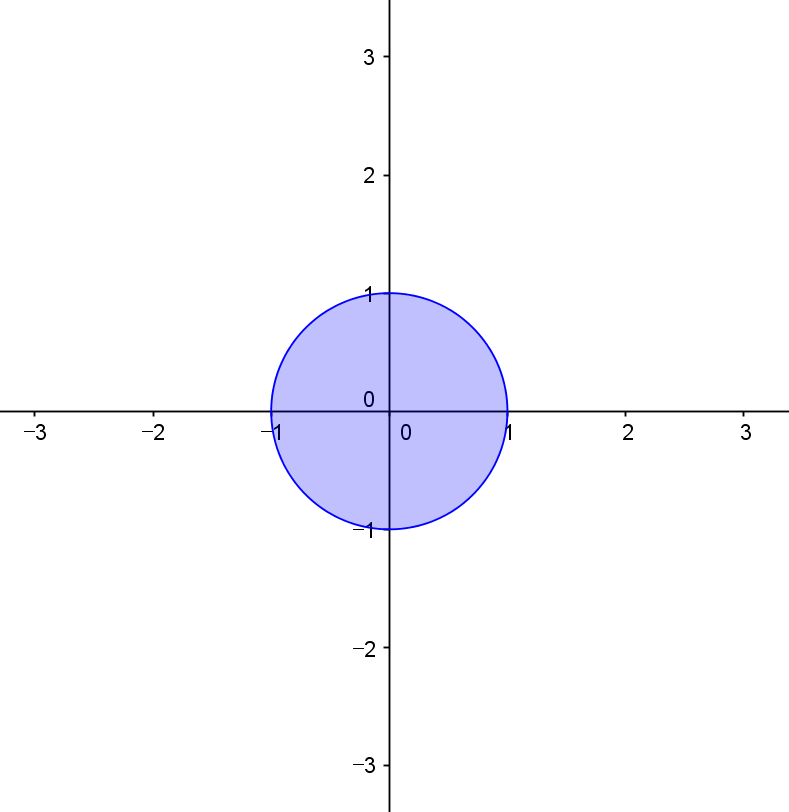
\includegraphics[width=0.3\textwidth]{2dimset1}&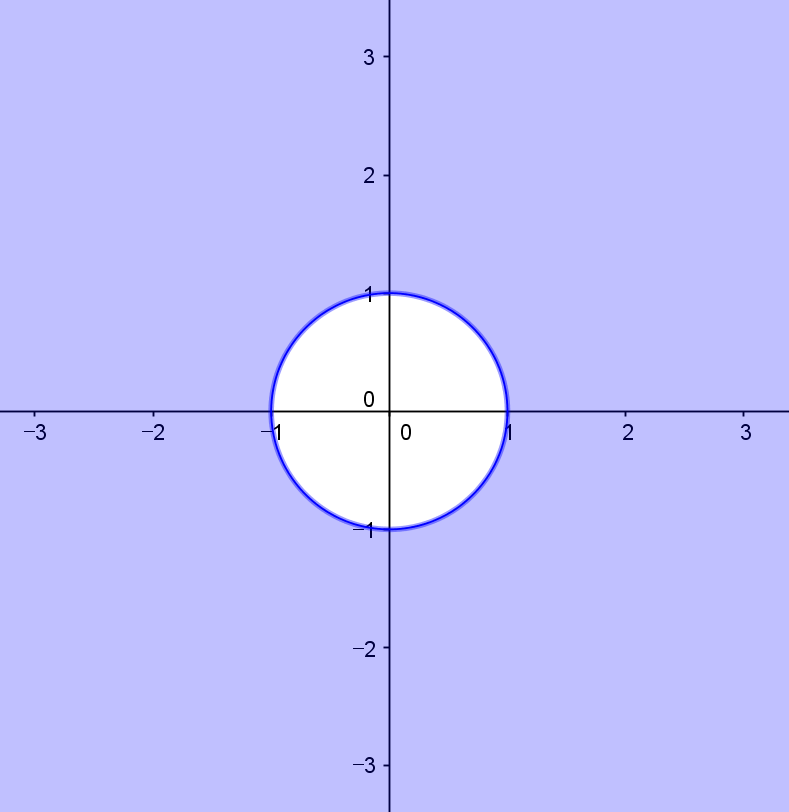
\includegraphics[width=0.3\textwidth]{2dimset2}
&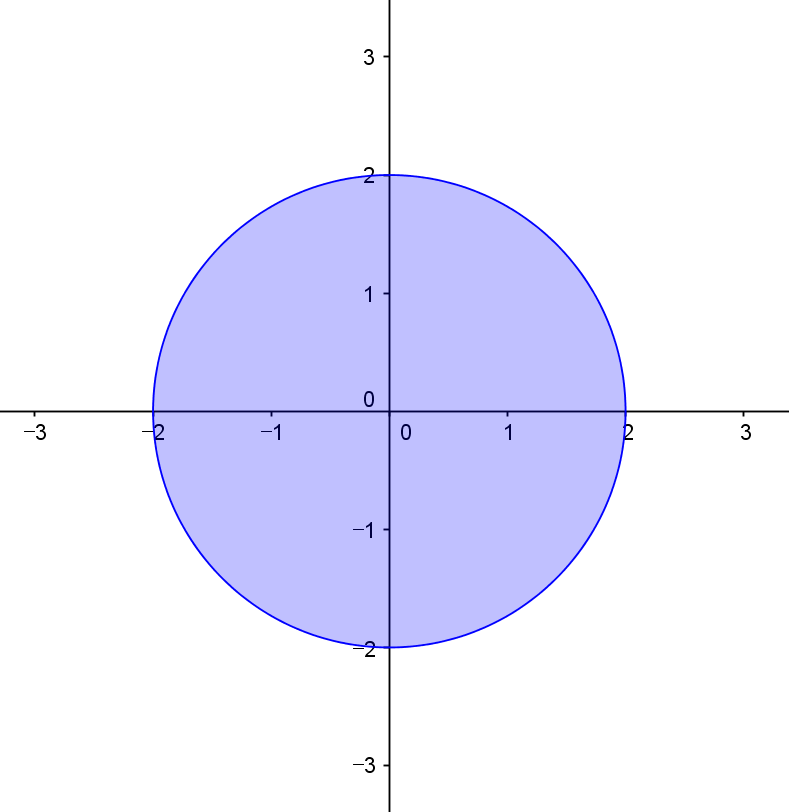
\includegraphics[width=0.3\textwidth]{2dimset3}\\
\ding{172}&\ding{173}&\ding{174}\\
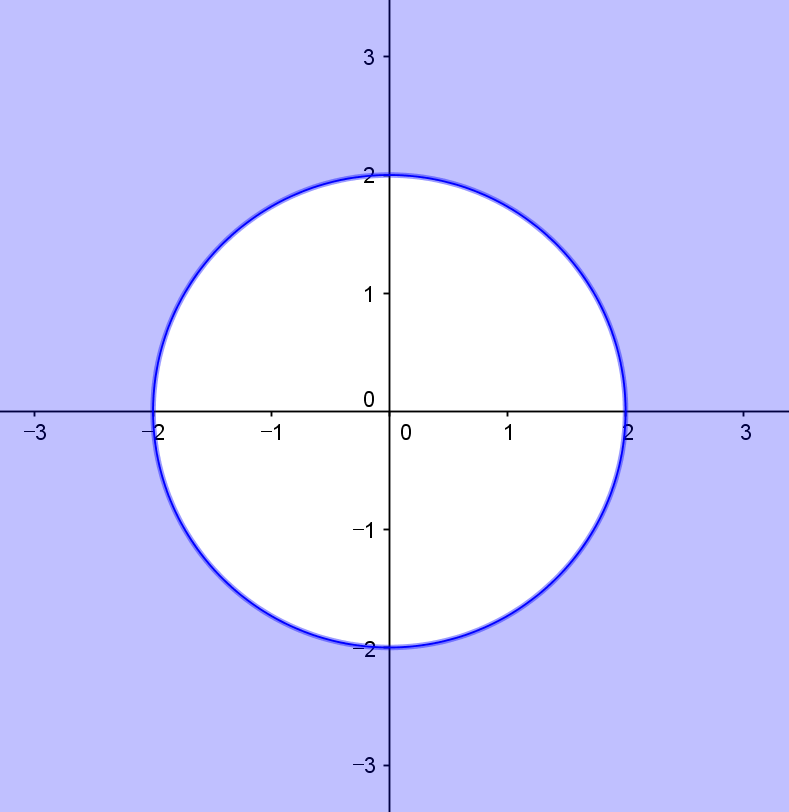
\includegraphics[width=0.3\textwidth]{2dimset4}&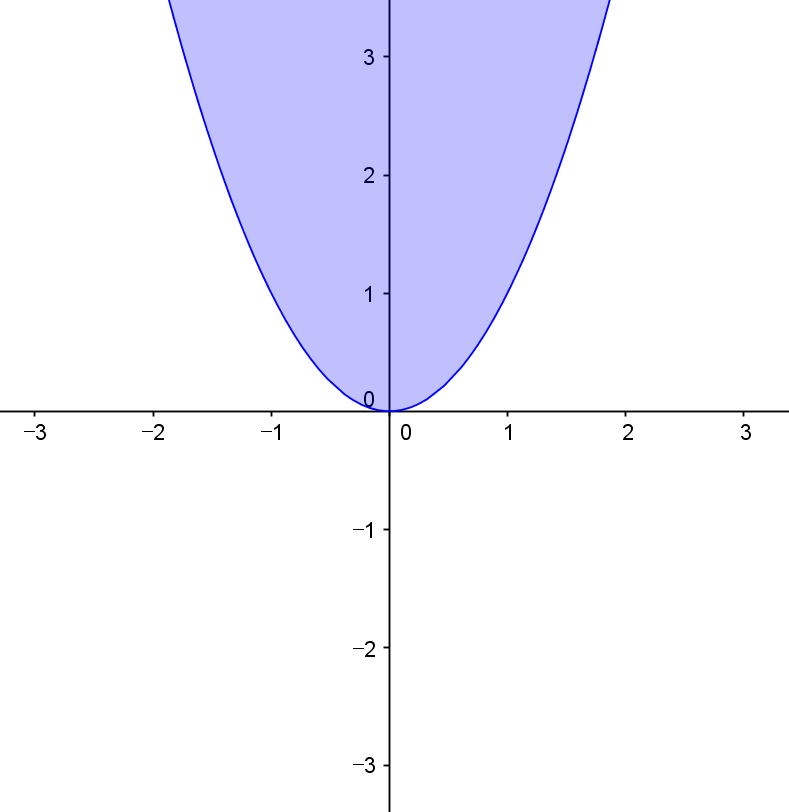
\includegraphics[width=0.3\textwidth]{2dimset5}\\
\ding{175}&\ding{176}\\
\end{tabular}

\clearpage
%
\prob{}
집합 \(A_n\), \(B_n\)이
\begin{align*}
A_n&=\{x\ba x\text{는 \(n\)의 약수}\}\\
B_n&=\{x\ba x\text{는 \(n\)의 배수}\}
\end{align*}
와 같이 정의될 때, 다음 중 틀린 것을 고르시오.
\tabb{2\in A_6}{3\notin A_1}{8\in B_4}{A_4\subset A_8}{B_4\subset B_8}
\end{document}